\section{Einleitung}
\label{sec:einleitiung}

Bei der Positionierung in Sensornetzen geht es darum, die Position
einzelner Sensoren herauszufinden. Dabei muss zwischen globaler und
lokaler Lokalisierung unterschieden werden. Die Lokalisierung der
einzelnen Sonsorknoten ist wichtig, da das Netzwerk sonst nicht weiß,
wo die entsprechenden Sensordaten herkommen und wie diese Daten
behandelt werden.

\begin{figure}[h!]
  \centering
  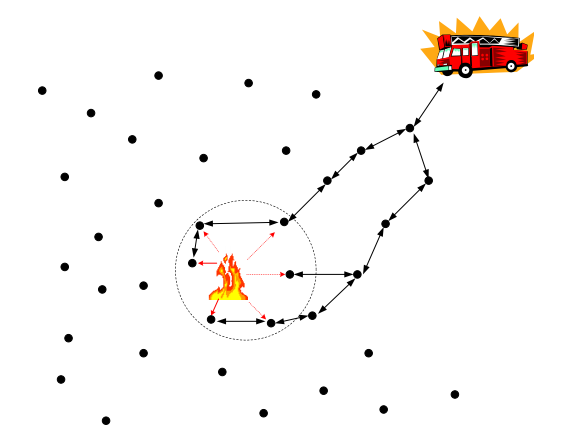
\includegraphics[scale=0.6]{img/lokalisierung_1}

  \caption{Beispiel für die Bedeutung der Lokalisierung in
    Sensornetzen}
  \label{fig:local}
\end{figure}

Abbildung \ref{fig:local} zeigt ein Sensornetz, in dem ein durch einen
Knoten ein Feuer gemeldet wird. Diese Information muss zur Zentrale
weiter geleitet werden, damit dort zum einen die Position des Feuers
bestimmt werden kann. Dafür müssen die Knoten die Position ihrer
Nachbarn kennen und die Position der Basis, damit die Information zum
einen an der richtigen Stelle ankommt. Des weiteren kann so auch der
kürzeste Pfad direkt in der Basis berechnet werden, wenn diese weiß,
wo die Daten herkommen und welche Sensoren sie dafür passiert haben.
\cite{gholami2011} 

Eines der größten Probleme bei der Lokalisierung besteht darin, dass
jedem Knoten nur sehr begrenzte Ressourcen zur Verfügung stehen.
Meistens verfügen diese über einen \ac{uC} der eine geringe
Rechenleistung und Speicherkapazität hat und zudem möglichst
stromsparend arbeiten muss. \cite{timmermann} Ein weiteres Problem
besteht darin, dass die Position von Knoten nicht stationär sein muss,
somit müssen die Berechnungen und Messungen direkt von den \ac{uC}'s
durchgeführte und wiederholt werden. \cite{roehrig2009} Dafür werden
bestimmte Verfahren und Algorithmen benötigt, wie die Abbildung
\ref{fig:algo} zeigt, die wir in dieser Ausarbeitung vorstellen und
diskutieren werden.

\begin{figure}[h!]
  \centering
  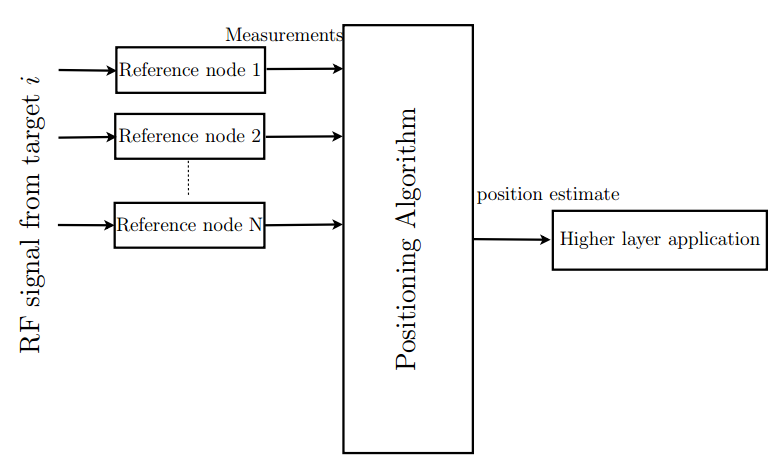
\includegraphics[scale=0.45]{img/algo_1}

  \caption{Darstellung des Zusammenhangs der Messung und Algorithmen}
  \label{fig:algo}
\end{figure}

